\documentclass{article}

\usepackage{url,graphicx,tabularx,array,geometry, hyperref}
\usepackage{listings}
\usepackage{fullpage}
\usepackage{fancyvrb}
\usepackage{framed}
\usepackage{lastpage}
\usepackage{fancyhdr}
\usepackage{float}

\renewcommand{\headrulewidth}{0pt}
\setcounter{secnumdepth}{0}

\setlength{\parskip}{1ex} %--skip lines between paragraphs
\setlength{\parindent}{0pt} %--don't indent paragraphs
\setlength{\headheight}{15.2pt}

\pagestyle{fancy}

\renewcommand{\headrulewidth}{0pt}
\lhead{  }
\lfoot{Lab 1: TCP Congestion Control}
\rfoot{page \thepage\ of \pageref{LastPage}}

\renewcommand{\familydefault}{\sfdefault}
\begin{document}

\begin{titlepage}
\begin{center}
\textsc{\huge \bfseries Advanced Networking 2018}\\[1.5cm]
\textsc{\large Lab \#1: TCP Congestion Control}\\[1.5cm]
\textsc{\huge Report}\\[1.5cm]
\textsc{\huge \bfseries GROUP: 1}\\[1.5cm]
\textsc{\large{\textbf{Authors:}\\ Rick van Gorp, rick.vangorp@os3.nl\\ Luc Gommans, os3@lucgommans.nl}}

\textsc{\large University of Amsterdam}
\end{center}
\end{titlepage}

\subsection{Q1.1 Plot a graph showing CWND versus time from 0.0s to 100.0s.}

\begin{figure}[H]
	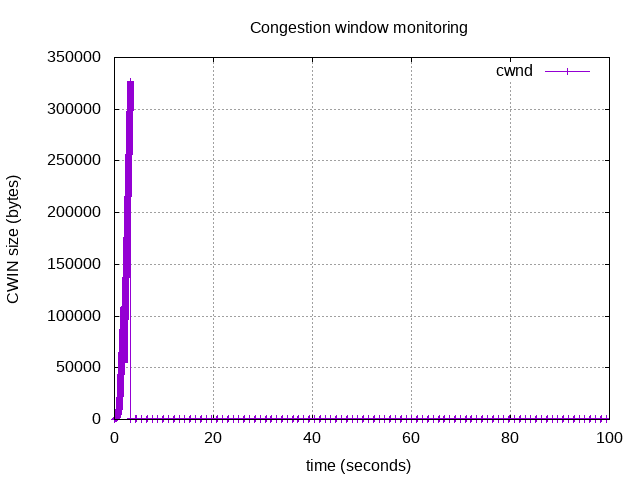
\includegraphics{lab1-group1-task1-question1.png}
	%\label{fig:dinges}
	\caption{T1Q1 CWND from 0 to 100 seconds}
\end{figure}


\subsection{Q1.2 Plot a graph showing SSTH versus time from 0.0s to 100.0s.}

\begin{figure}[H]
	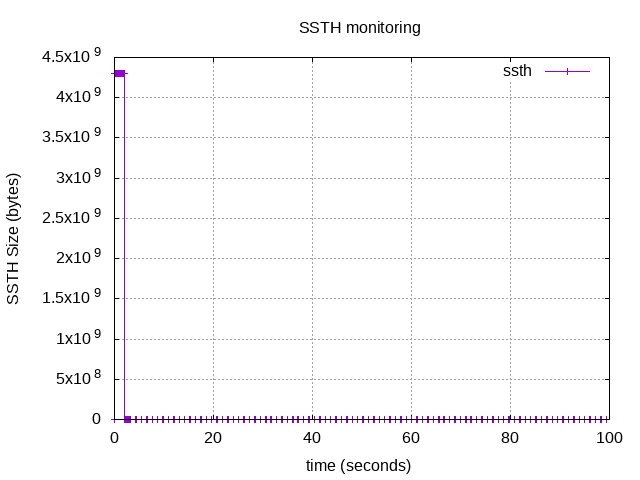
\includegraphics{lab1-group1-task1-question2.png}
	%\label{fig:dinges}
	\caption{T1Q2 SSTH from 0 to 100 seconds}
\end{figure}


\subsection{Q1.3 Find the points where the slow-start, congestion-avoidance, fast retransmit/fast recovery states begin.}
Table \ref{table:results1} shows the points where the slow-start, congestion-avoidance and fast recovery states begin.
The results are based on the reno datafiles generated in the vagrant boxes and the states described in the slidedeck of lecture 1.
We found the slow-start state starts at 0 seconds and is followed by the fast recovery state as $ssthresh$ halves and $cwnd$ becomes 3 higher than $ssthresh$.
After the fast recovery state we see that the algorithm goes to the slow start state again and then, after some time $cwnd$ exceeds $ssthresh$. From here the transition from slow start to congestion-avoidance occured.

\begin{table}[H]
\center
\caption{Points of state transitions NewReno algorithm}
\label{table:results1}
\begin{tabular}{|c|p{25mm}|p{20mm}|c|c|}
\hline Time (s)    & Current CWND (bytes)    & New CWND (bytes)    & New State             & Event            \\
\hline 0.00000     & 0                       & 340                 & slow-start            & start            \\ 
\hline 1.93189     & 109 480                 & 55 590              & fast-recovery         & dupACKcount==3   \\ 
\hline 3.26916     & 326 570                 & 340                 & slow-start            & timeout          \\ 
\hline 3.30286     & 340                     & 680                 & congestion-avoidance  & cwnd$>=$ssthtresh  \\ 
\hline  
\end{tabular} 
\end{table}


\subsection{Q1.4 Plot a graph showing CWND versus time from 0.0s to 100.0s.}

\begin{figure}[H]
	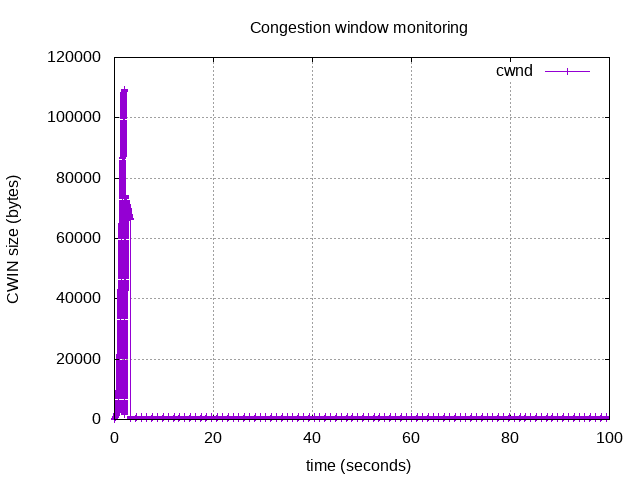
\includegraphics{lab1-group1-task1-question4.png}
	%\label{fig:dinges}
	\caption{T1Q4 CWND from 0 to 100 seconds}
\end{figure}


\subsection{Q1.5 Plot a graph showing SSTH versus time from 0.0s to 100.0s.}

\begin{figure}[H]
	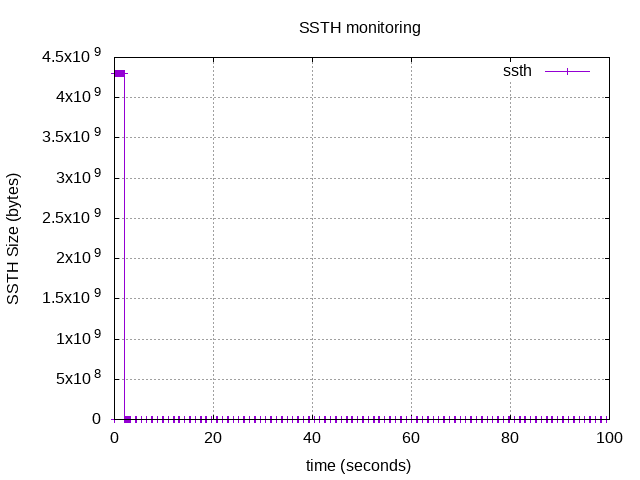
\includegraphics{lab1-group1-task1-question5.png}
	%\label{fig:dinges}
	\caption{T1Q5 SSTH from 0 to 100 seconds}
\end{figure}


\subsection{Q1.6 Find the points where the slow-start, congestion-avoidance, fast retransmit/fast recovery states begin.}

TODO

\begin{table}[H]
\center
\caption{Points of state transitions WestWood algorithm}
\label{table:results2}
\begin{tabular}{|c|p{25mm}|p{20mm}|c|c|}
\hline Time (s)    & Current CWND (bytes)    & New CWND (bytes)    & New State             & Event            \\
\hline 0.00000     & 0                       & 340                 & slow-start            & start            \\ 
\hline 1.21176     & 163 882                 & 82 790              & fast-recovery         & dupACKcount==3   \\ 
\hline ???????     & 326 570                 & 340                 & slow-start            & timeout          \\ 
\hline 2.54903     & 151 810                 & 340                 & fast-recovery         & TODO \\ 
\hline  
\end{tabular} 
\end{table}


\subsection{Q1.7 Discuss and motivate the differences you observe between the NewReno and this algorithm.}

TODO

\subsection{Q2.1 Plot a graph showing the CWND and ssthresh versus time with all the data you get. These two metrics are in one graph.}\label{sec:q21}

\begin{figure}[H]
	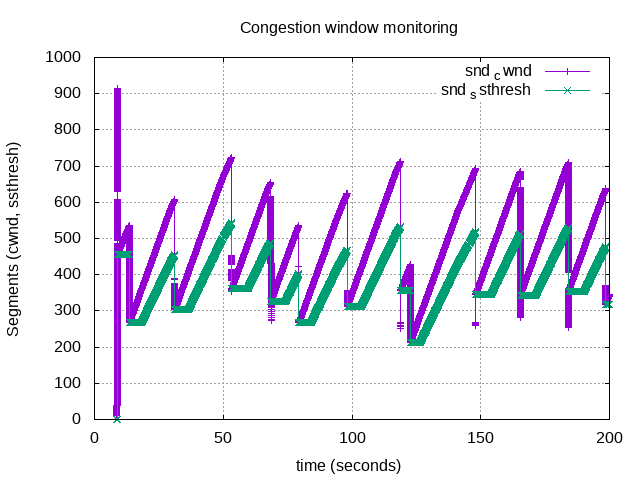
\includegraphics{lab1-group1-task2-question1.png}
	\label{fig:q21}
	\caption{T2Q1 CWND and ssthresh 0 to 200 seconds}
\end{figure}


\subsection{Q2.2 Briefly discuss the changing process.}

We see that it initally starts in slow start, until the source received three
duplicate ACKs. It then transitions to fast recovery, where it slowly increases
the congestion window until it receives a new ACK. We are now in congestion
avoidance. From there we see multiple transitions between congestion avoidance
and fast recovery, as we see the threshold halving and the CWND is adjusted to
\texttt{ssthresh + 3MSS}.


\subsection{Q2.3 Plot a graph showing CWND versus time with all the data you get.}

\begin{figure}[H]
	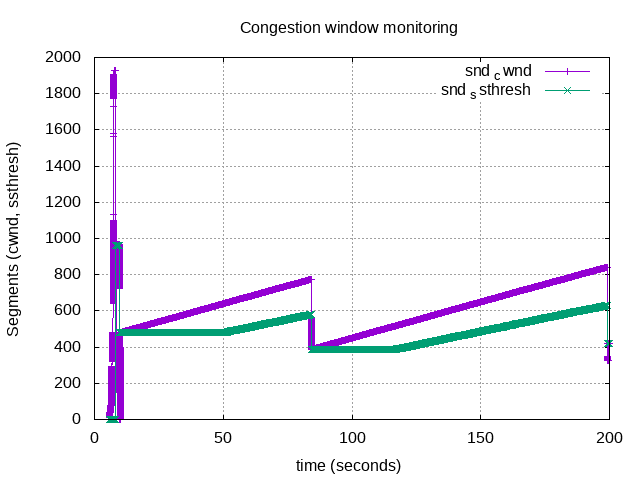
\includegraphics{lab1-group1-task2-question3.png}
	\label{fig:q23}
	\caption{T2Q3 CWND and ssthresh 0 to 200 seconds}
\end{figure}


\subsection{Q2.4 Compare this graph with the one from}

Both graphs start similarly. The relatively fast, oscillating changes between
the fast recovery and congestion avoidance states, are much slower in the
latter (figure \ref{fig:q23}). The congestion avoidance states in figure \ref{fig:q23} hold for a longer time than in figure \ref{fig:q21}. 


\subsection{Q2.5 Plot a graph showing CWND and ssthresh versus time with all the data you get.}

\begin{figure}[H]
	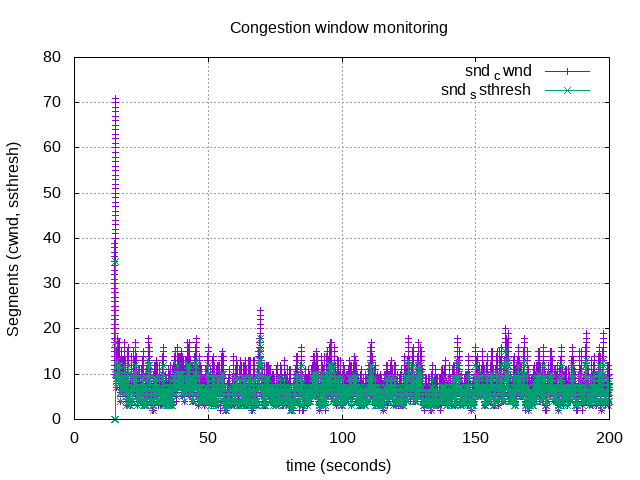
\includegraphics{lab1-group1-task2-question5.png}
	\caption{T2Q5 CWND and ssthresh 0 to 200 seconds with packet loss}
	%\label{fig:dinges}
\end{figure}


\subsection{Q2.6 Compare this graph with the graph of}

In this graph, the congestion window never reaches the same levels as in
previous exercises. At the peak of slow start, it is just over $70*MSS$. Here
we see a very fast oscillation between fast recovery and congestion avoidance.
It does not go back to slow start, because it never starts again with 1MSS.
This implies the throughput is much lower than in subsection \ref{sec:q21}.


\subsection{Q2.7 Zoom in the graph of this scenario (plot some parts of this scenario in a short duration, 10 or 20 seconds). Briefly explain the changing process.}

\begin{figure}[H]
	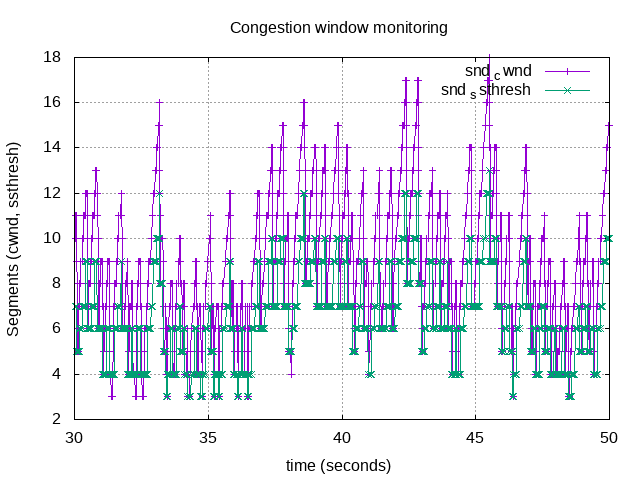
\includegraphics{lab1-group1-task2-question7.png}
	\caption{T2Q7 CWND and ssthresh 0 to 200 seconds with packet loss zoomed in}
	%\label{fig:dinges}
\end{figure}

Due to the relatively high percentage of packet loss, this connection is quite
unstable. We see the same pattern as previously, oscillating between congestion
avoidance and fast recovery, but the lowest points are as much as 8 times lower
than the peaks. Previously, the highest difference observed was around 2.8
times.


\subsection{Q2.8 Show a screen capture of the real throughput in this scenario.}

\begin{figure}[H]
	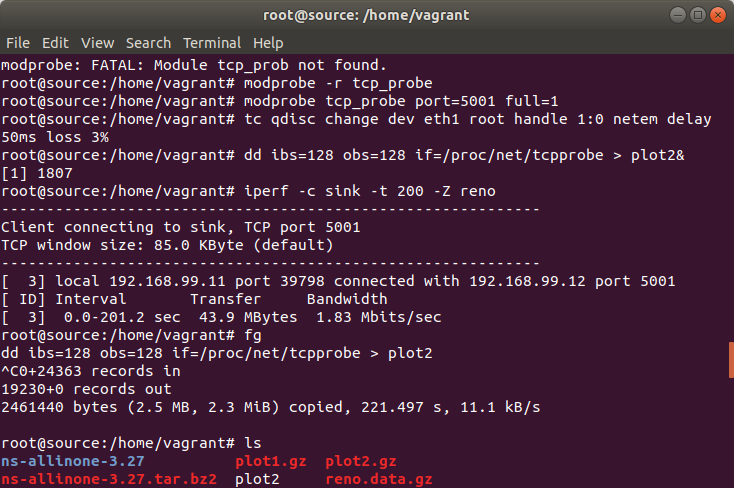
\includegraphics[width=0.8\textwidth]{lab1-group1-task2-question8.png}
	%\label{fig:dinges}
	\caption{T2Q8 Throughput of Reno algorithm}
\end{figure}


\subsection{Q2.9 Plot a graph showing CWND and ssthresh versus time with all the data you get.}

\begin{figure}[H]
	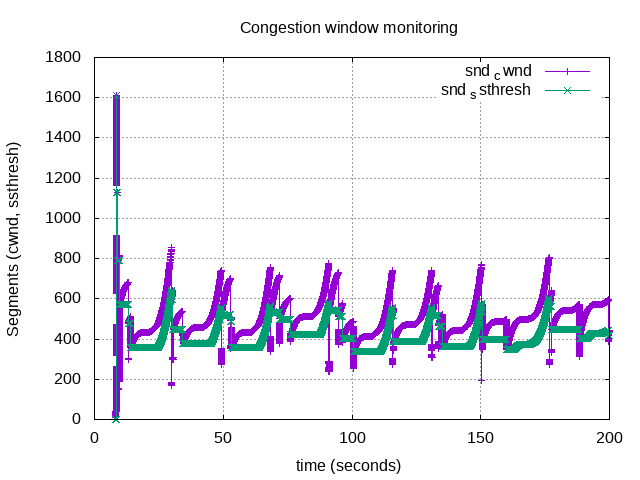
\includegraphics{lab1-group1-task2-question9.png}
	\caption{T2Q9 CWND and ssthresh 0 to 200 seconds (CUBIC)}
	%\label{fig:dinges}
\end{figure}


\subsection{Q2.10 Compare this graph with the graph of}

The main difference which catches the eye, is that it has differently-shaped,
smooth curves in the congestion window. When looking up how CUBIC works, we see
this pattern explained many times as being fast growth upon reduction on a
packet loss event, and slower probing for the maximum throughput.


\subsection{Q2.11 Plot a graph showing CWND and ssthresh versus time with all the data you get.}

\begin{figure}[H]
	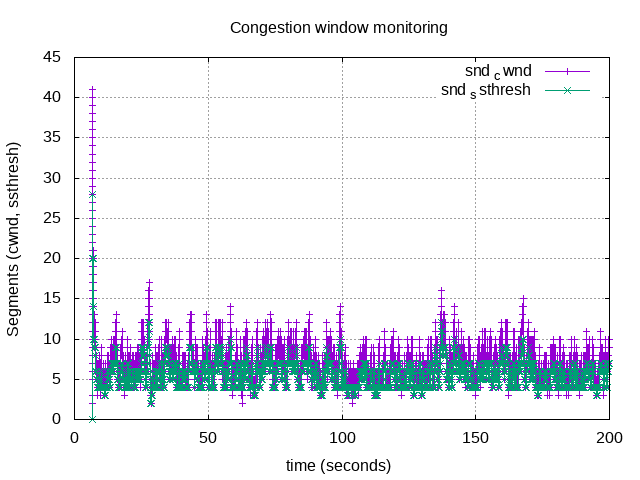
\includegraphics{lab1-group1-task2-question11.png}
	\caption{T2Q11 CWND and ssthresh 0 to 200 seconds (CUBIC) with packet loss}
	%\label{fig:dinges}
\end{figure}


\subsection{Q2.12 Compare this graph with the graph of scenario three and show the differences.}

CUBIC generally seems less aggressive. In the slow start state, it does not
reach as high as Reno ($42*MSS$ versus $71*MSS$). In the later states, it
decreases less far and usually goes down to $4*MSS$ or sometimes $3*MSS$. Reno
shows more fluctuations than CUBIC; therefore, CUBIC seems to be more stable in
those circumstances.


\subsection{Q2.13 Zoom in the graph of this scenario (plot some parts of this scenario in a short duration, 10 or 20 seconds). Briefly explain the changing process and compare it with the graph of}

\begin{figure}[H]
	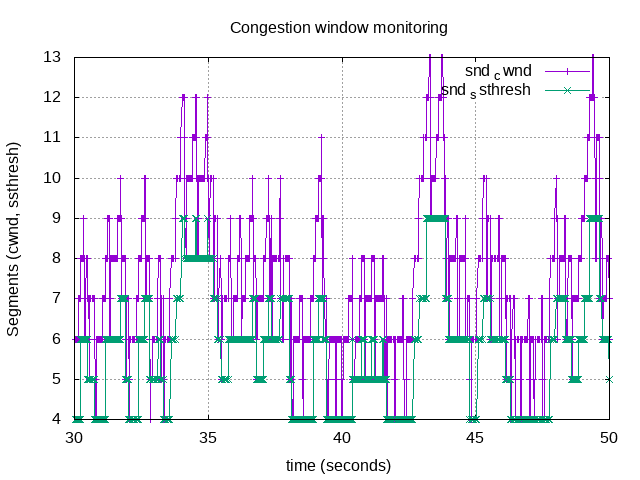
\includegraphics{lab1-group1-task2-question13.png}
	\caption{T2Q13 CWND and ssthresh 0 to 200 seconds (CUBIC) with packet loss zoomed in}
	%\label{fig:dinges}
\end{figure}

Here, too, we see that CUBIC is more stable than reno. The difference between
the minimum and maximum value, is higher in Reno. The frequency of the state
changes is also higher in Reno.


\subsection{Q2.14 Show a screen capture of the real throughput and compare it with throughput of}

\begin{figure}[H]
	%\caption{dinges}
	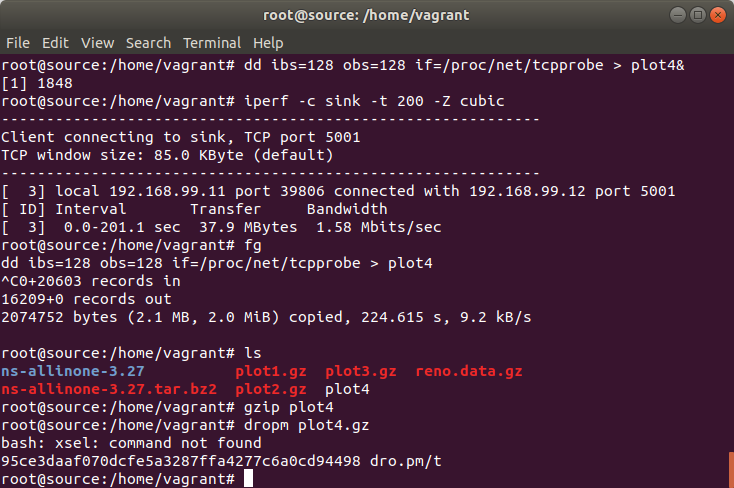
\includegraphics[width=0.8\textwidth]{lab1-group1-task2-question14.png}
	\caption{T2Q14 Throughput of CUBIC algorithm}
	%\label{fig:dinges}
\end{figure}

Reno has a higher throughput than CUBIC.


\subsection{Q3.1 Explain what an LFN network is. Change the simulation parameters to your likings and demonstrate that TcpNewReno is not suitable for LFN networks.}

\subsection{Q3.2 Explain SACK does. Change the simulation parameters to your likings and demonstrate the performance improvement with SACK.}

\subsection{Q3.3 Explain with TCP fairness is. Show the effect of multiple flows in the simulation.}

\subsection{Q3.4 Replicate scenario 3 of the emulation: packet loss of 3\%, delay of 50 ms and transfer duration of 200sec. Use TcpNewReno. Compare the two results.}

\subsection{Q3.5 After these experiments, please briefly describe the difference between simulation and emulation?}

\end{document}
